% 例子环境
\begin{example}

\end{example}

% 表格环境
\begin{table*}[]
    \centering
    \resizebox{0.7\linewidth}{!}{
        \begin{tabular}{c | c | c | c}
            
        \end{tabular}
        }
        \bicaption{柱形延拓-区间计算。} {Demo of Computation of Cylindrical Expansion-Interval Splitting.}
\label{tab:expansion}
\end{table*}

% 图片环境
\begin{figure*}[t]
    \centering
    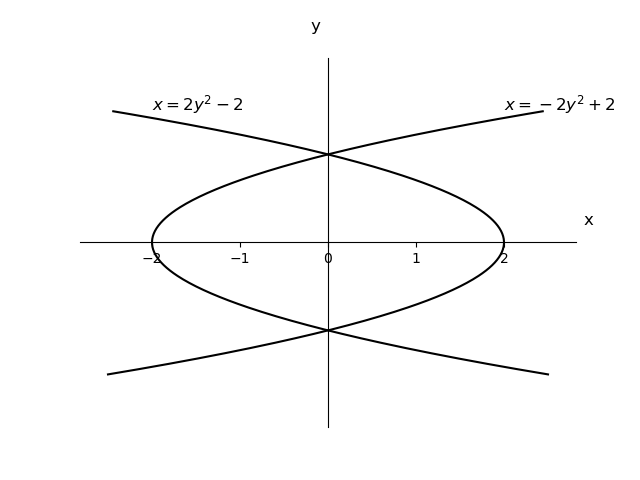
\includegraphics[width=\columnwidth]{Img/cad.png}
    \bicaption {柱形代数分解步骤示意图。} {Demo of Cylindarical Algebraic Decomposition Steps.}
\label{fig:CAD}
\end{figure*}


% 定义环境
\begin{definition}[\textbf{AllDifferent约束图}]
    异构图被定义为$\mathcal{G} = (V, E)$,其中$V = X\cup NV$,表示顶点集合,其中$NV$指出现在AllDifferent约束中的变量表达式集合。
    $E = E_p \cup E_x$表示边集合,它由两种类型的边表示。
    具体来说,一种类型是变量表达式之间的边,称为\textit{表达边},用$E_p$表示,如果两个变量表达式$p$和$q$出现在同一个AllDifferent约束中,它表示为$(p, q) \in E_p$。
    另一种类型是变量和变量表达式之间的边,用$E_x$表示,如果一个变量表达式$p$包含一个变量$x$,则有$(p, x) \in E_x$。
\end{definition}

% 算法环境
\begin{algorithm}[t]
    % \small
    \caption{$SelectSolution$ function}
    \label{alg:SelectSolution}
    \textbf{输入}: An ACG $\mathcal{G}(V,E)$, a complete assignment $C$ and a solution pool $\mathcal{AC}$\\
    \textbf{输出}: A complete assignment $\mathcal{A}'$
    
    \begin{algorithmic}[1] %[1] enables line numbers
        \Statex \hrulefill
        \STATE $\mathcal{A}.step \leftarrow \alpha$;
        \IF {$\mathcal{AC} = \emptyset$ \textbf{or} $cost(\mathcal{G}, \mathcal{A}) < \mathcal{AC}.cost$}
            \STATE Reset $e.w$ for $\forall e \in E_p$;
            \STATE $\mathcal{AC} \leftarrow \{\mathcal{A}\}$;
            \STATE $\mathcal{AC}.cost \leftarrow cost(\mathcal{G},\mathcal{A})$;
            \STATE Update $e.w$ ($e \in E_p$) based on weight strategy;
        \ELSIF {$cost(\mathcal{G}, \mathcal{A}) = \mathcal{AC}.cost$}
            \IF {$\mathcal{A} \neq \mathcal{A}'$ \textbf{for} $\forall \mathcal{A}' \in \mathcal{AC}$}
                \STATE $\mathcal{AC} \leftarrow \mathcal{AC} \cup \{\mathcal{A}\}$;
                \STATE Update $e.w$ ($e \in E_p$) based on weight strategy;
            \ELSE
                \STATE $\mathcal{A}'.step \leftarrow A'.step + \gamma * \alpha$;
            \ENDIF
        \ENDIF
        \STATE Update $\mathcal{AC}$ based on its size and weight strategy;
        \STATE Select a $\mathcal{A}'$ from $\mathcal{AC}$ randomly;
        \STATE Disturb $\mathcal{A}'$ based on disturbance strategy;\\
        \RETURN $\mathcal{A}'$
    \end{algorithmic}
\end{algorithm}